\documentclass[12pt,extarticle]{article}

% Packages
\usepackage[left=24mm, top=24mm, right=24mm]{geometry}
\usepackage{color}
\usepackage{listings}
\usepackage{graphicx}
\usepackage{hyperref}

% Declaring Colors
\definecolor{codebg}{RGB}{255, 255, 238}
\definecolor{codeborder}{RGB}{243, 242, 222}
\definecolor{purple}{RGB}{174, 19, 198}
\definecolor{darkblue}{RGB}{0, 0, 102}
\definecolor{lightblue}{RGB}{50, 155, 171}
\definecolor{lightgreen}{RGB}{29, 131, 43}

% Declaring style for code blocks (dstyle).
\lstdefinestyle{dstyle} {
	backgroundcolor=\color{codebg},
	rulecolor=\color{codeborder},
	stringstyle=\color{purple},
	keywordstyle=\color{darkblue},
	identifierstyle=\color{lightblue},
	commentstyle=\color{lightgreen},
	basicstyle=\footnotesize\sffamily,
	xleftmargin=10pt,
	xrightmargin=10pt,
	belowcaptionskip=10pt,
	belowskip=20pt,
	framesep=10pt,
	frame=single,
	%numbers=left,
	%numbersep=8pt,
	showspaces=false,
	showstringspaces=false,
	tabsize=2
}

% Sets the style for code blocks.
\lstset {
	style=dstyle
}

% Document information.
\title{\textbf{CS 136 Midterm Review Notes}}
\author{Jacob Pollack}
\date{}

% Document formatting.
\pagestyle{headings}

% Fonts and other stuff.
\sffamily

% Hyperlink setup.
\hypersetup {
    colorlinks=false,
    pdfborder={0 0 0}
}

% Table of Contents
\renewcommand{\contentsname}{Table of Contents}

% New commands (strings).
\newcommand{\docauthor}{Jacob Pollack}
\newcommand{\docbuild}{1.06}

% Begin the document.
\begin{document}

\thispagestyle{empty}

\makeatletter
\hfil\parbox[t]{0.7\textwidth}{\centering\LARGE\bfseries\@title}\par
\kern0.5cm \hrule\kern0.5cm
\makeatother

\section*{Preamble}
This document (build \docbuild) will outline my perspective of the pre-midterm material covered in CS 136 during the summer semester of 2013. It is not aimed to replace lectures or your own studying, it is aimed to be a study aid that you can refer to. These notes will be provided under no warranty of accuracy or maintainability. If you are confused on a topic, refer to the actual course material, Piazza or meet with your professor for a further (and more accurate) explanation of a topic.\\

My review notes were written during the University of Waterloos' summer semester offering of CS 136. It covers only pre-midterm material (modules 1 - 5). The professors during this time were: Dave Tompkins, Olga Zorin and Patrick Nicholson.\\

The course material that influenced the contents of these review notes are:

\begin{itemize}

\item Lecture slides designed by the professors.
\item "C Programming a Modern Approach - Second Edition", textbook for the course.
\item CS 136 on Piazza.
\item and other third party websites used to improve my understanding.

\end{itemize}

I ({\docauthor}, student at the University of Waterloo) created this review notes document. The material this document contains are my review notes for the midterm. I went through every page in the lecture slides and assigned readings to highlight what I think is important. That highlighted information can be found here, there will be strong paraphrasing with a mix of my own perspective of the material.\\

To preserve the chronological order that the material was taught in, my review notes are written in the same order. I may have switched around material to introduce it sooner or later to have a different flow. I may have also added or removed content that I felt needed an extra emphasis or was not too important.\\

I have included some exercises for topics I thought my peers (including myself) struggled on. To determine these topics I lurked Piazza for a couple hours to find the most common help posts. These exercises are found after the review (page 47).\\

\textbf{I am in no way, shape or form claiming these notes are accurate. They are my perspective of the pre-midterm material. These were designed to test if I knew the material through attempting to explain it.}

\newpage
\thispagestyle{empty}
\section*{Disclaimer}
I am only going to ask a few things that I hope everyone respects. Please be aware of the academic integrity rules set forth by the University. These review notes are in no way a replacement of content for your respective semesters' offering of CS 136, they are merely a study aid.\\

I alone reserved the right to alter and distribute these notes. You are not allowed to do either. If you see a mistake or feel as if content should be added, contact me so that I can make the appropriate correction(s). I will be supporting the accuracy of these notes for the remainder of the summer semester. After such a time these review notes should be considered obsolete. The latest build of these review notes can be found at the following link:\\

\textbf{www.jamach.com/cs136/review\_notes\_updated.pdf} (with the underscores).\\

I have attempted to acknowledge all sources in the preamble. If I missed an acknowledgement or if you feel as if an acknowledgement should be explicit with a corresponding word, phrase or paragraph, send me an e-mail and I will add it.\\

These review notes are provided absolutely free of charge. If you paid for or downloaded a copy of these notes from anywhere other than the groups on Facebook for the University of Waterloo then you are obligated to report this to me! Such activity is shamed upon.\\

You can reach me at my student e-mail \textbf{jpollack@uwaterloo.ca} or jacobpollack@jamach.com.

\section*{Special Notices}

This document would not be possible without the offering of CS 136 at the University of Waterloo. It is truly an amazing course and I am absolutely loving it. I would like to make a note on peers that contributed towards the result of this review package. Special thanks to:\\

\begin{itemize}

\item Jacob Willemsma.
\item Nimesh Das.

\end{itemize}

\newpage
\thispagestyle{empty}
\tableofcontents

\newpage
\section{Introduction: Module 01}

This course is described by the University of Waterloo as follows \emph{"... builds on the techniques and patterns learned in CS 135 while making the transition to use of an imperative language. It introduces the design and analysis of algorithms, the management of information, and the programming mechanisms and methodologies required in implementations. Topics discussed include iterative and recursive sorting algorithms; lists, stacks, queues, trees, and their application; abstract data types and their implementations."}. I do not think this will be asked on the midterm, however I felt that this should give you a brief understanding of what we are expected to know by the end of this course.\\

In the prerequisite course(s) -- CS 135, CS 115/116, the focus was programming in a functional paradigm. Programming in a \textbf{functional paradigm} is the process of evaluating code as a sequence of Mathematical functions, avoiding mutation and state (no not X-Men mutation). In this course we are required to program in both a functional paradigm and in an \textbf{imperative paradigm}. There is a third paradigm called declarative programming, however we do not have to worry about it and hence it will not be referenced again in my review.\\

Now you are probably asking yourself, what is the \textbf{difference between programming in a functional and imperative paradigm}? We now know that programming in a functional paradigm avoids mutation and state. Hence we commonly achieve our goals through recursion. However in an imperative paradigm, we use mutation and change the state of our program frequently -- giving us a lot more freedom to accomplish a given task. Here are two examples of summing the numbers from [0, n]. The first example is programming in a functional paradigm, however the second example is programming in an imperative paradigm.\\

\lstset {
	language=C
}
\begin{lstlisting}
int sum( int n ) {
	return ( 0 == n ) ? n : ( n + sum( n - 1 ) );
}
\end{lstlisting}

\lstset {
	language=C
}
\begin{lstlisting}
int sum( int n ) {
	int acc_sum = 0;
	
	for ( int i = 0; i <= n; i++ ) {
		acc_sum += i;
	}
	
	return acc_sum;
}
\end{lstlisting}

For the time being we will be required to program in a functional paradigm. We will be visiting imperative programming in module 05.

\subsection{Full Racket}

It is true! We are finally old enough (as Dave says) to use full Racket. To enable full Racket, you should have the following declaration at the top of every Racket file.\\

\lstset {
	language=Lisp
}
\begin{lstlisting}
#lang racket
\end{lstlisting}

Keep in mind there is some funky terminology for Racket. We \textbf{apply} functions, which \textbf{consumes} arguments and \textbf{produce} a value. In the following example, \textbf{x} and \textbf{y} are \textbf{parameters}.\\

\lstset {
	language=Lisp
}
\begin{lstlisting}
(define (f x y)
	(sqr (+ x y))
\end{lstlisting}

Recall what a \textbf{constant} is? When you declare a constant, it is an immutable identifier in Racket (however not always). Constants are quite useful when it comes to readability and maintainability (which will be discussed later). An example:\\

\lstset {
	language=Lisp
}
\begin{lstlisting}
(define penny 1)

(define (value-of-n-pennies n)
	(* n penny))
\end{lstlisting}

But that does not make sense... there is only one money penny :p (joking)\\

In Full Racket we can now declare functions without parameters. A keen observer will notice that their declaration is very similar to the declaration of a constant, however do not fool yourself. They are very different! An example:\\

\lstset {
	language=Lisp
}
\begin{lstlisting}
; Declaring a constant.
(define some-constant 9)

; Declaring a function without parameters.
(define (some-function) 9)

; Something wacky.
(define (do-something-wacky n)
	(+ n (* some-constant (some-function))))
\end{lstlisting}

Recall what a \textbf{top-level expression} is from CS 115/135. They are expressions that are evaluated at the top-level when you run your Racket program. Racket will display the result of each top-level expression in the console window. Here is an example of everything we have learned thus far in Racket (excluding structures):\\

\lstset {
	language=Lisp
}
\begin{lstlisting}
#lang Racket ; my-file.rkt

; Some top level expression.
(+ (+ 3 3) 3) ; => 9
(* 2 2)       ; => 4

; Declaration of a constant.
(define x 9)

; Declaration of functions.
(define (no-param-func)
	...)

(define (some-func x y z)
	...)
\end{lstlisting}

There are a few more things we should be able to recall: booleans, symbols, strings, characters, logical operators (and ... or) and conditional statements. I will not be going over this as they are pretty trivial. \textbf{Fun fact}, 0 is not false in Racket. However there is a new notation we are introduced to for condition statements. The old and newer notation is provided below:\\

\lstset {
	language=Lisp
}
\begin{lstlisting}
; Old notation (still useful).
(cond
	[q1 a1]
	[q2 a2]
	[else a3])

; New notation.
(if expression answer-true answer-false)
\end{lstlisting}

Structures in Racket have always been tricky for me to syntactically remember. With the introduction of full Racket it has become even harder. Originally structures could be output to the console and it would display their contents as-is. However in full Racket structures are not displayed to the console without a special keyword, \textbf{transparent}. An example of how to declare a structure posn with the older and newer syntax:\\

\lstset {
	language=Lisp
}
\begin{lstlisting}
; Older syntax.
(define-struct posn (x y))

; Newer syntax.
(struct posn (x y) #:transparent)
\end{lstlisting}

You should be able to recall what a list is in Racket. There are two new functions we are permitted to use: \textbf{last} and \textbf{drop-right}. In full Racket the function \textbf{member} behaves differently. If an element, e is a member of the list, it will produce the tail of the list starting at the first occurrence of e, otherwise false. To show an example:\\

\lstset {
	language=Lisp
}
\begin{lstlisting}
(member 9 (list 1 3 9 27 81)) ; => '(27 81)
(member 5 (list 1 3 9 27 81)) ; => #f
\end{lstlisting}

Another feature full Racket that is mainly for convenience is, we are able to \textbf{implicitly declare local functions and constants}. An example will not be provided.

\subsection{Binary Search Trees (BST)}

No unfortunately these are not going away. I know, take a moment if you must and then return to this review... :(\\

Binary Search Trees (henceforth referenced as BSTs) will be an integral part of our experience as a CS student at the University of Waterloo. To review some terminology, the first \textbf{node} is called the \textbf{root node}. Each node points to two \textbf{child nodes}. The left child node must be less than or equal to the index of the parent node and the right child node must be greater than or equal to the index of the parent node -- this is known as the \textbf{ordering property}. If a node does not have a left or right child node, it is commonly referred to as a \textbf{leaf}. Below are a couple examples of BSTs.\\

\lstset {
	language=Lisp
}
\begin{lstlisting}
; Declaring the structure of a BST.
(struct bst-node (key val left right) #:transparent)

; Declaring a BST.
(define bst (make-node 10 "" (make-bst-node 8 "" empty empty)
                             (make-bst-node 12 "" empty empty)))
\end{lstlisting}

Since BSTs can be very annoying and hard to understand, I provided another example of an implementation for a function that will produce the true or false if a given key \emph{k} is in a given BST \emph{abst}. The declaration of the BST structure is omitted for the example.\\

\lstset {
	language=Lisp
}
\begin{lstlisting}
; Declaring the structure of a BST.
(struct bst-node (key val left right) #:transparent)

(define (exists-key? k abst)
	(cond
		[(empty? abst) #f]
		[(equal? k (bst-node-key abst)) #t]
		[else (or (exists-key? k (bst-node-left abst))
		          (exists-key? k (bst-node-right abst)))]))
\end{lstlisting}

\subsection{Abstract List Functions and Lambda}

You should be able to recall what an \textbf{abstract list} function is from your experience in CS 135 or CS 115/116. For convenience I will list the ones we have been using often on assignments (and will likely be needed for the midterm). Some abstract list functions include: \emph{filter}, \emph{build-list}, \emph{map}, \emph{foldr} and \emph{foldl}.\\

These next few paragraphs and examples are going to outline my favorite feature in Racket. The feature is called an anonymous function, more commonly referred to as \textbf{lambda}. This is an extremely, exxtremely, exxxtremely powerful feature in Racket. An anonymous functions allows us to declare functions without names. This may not be obvious for why it is useful at first, however take a look at these uses of lambda.\\

\lstset {
	language=Lisp
}
\begin{lstlisting}
; Declaring a sample list.
(define sample-list '(1 2 3 4 5 6 7 8 9 10))

; Some uses of lambda.
(filter (lambda (x) (and (even? x) (> x 5))) sample-list) ; => '(6 8 10)

(build-list 5 (lambda (x) (* x x))) ; => '(0 1 4 9 16)
\end{lstlisting}

\subsection{Documentation (Design Recipe)}

This is a very tedious but necessary part of designing successful software. I am almost certain we will be tested for how well we document our code on the midterm (unless it specifies to omit this step due to time constraints). From assignments 1 - 5 we have only had a few hand marked questions, however documentation is required none the less.\\

The main goal of the design recipe is to aid in communicating what your function should consume, what it will achieve and what are its constraints. Once we get further into modularization you will see it is extremely important to maintain well documented code. Recall from CS 115/135 that there were quite a few elements to the design recipe. In CS 136 we only need to worry about 4. These elements are referred to as the \textbf{contract}, \textbf{purpose} and \textbf{pre} and \textbf{post conditions}.\\

Recall the sum function I wrote on page 2 of this document? If it were in Racket, the design recipe would be as follows:\\

\lstset {
	language=Lisp
}
\begin{lstlisting}
; (sum n): Int -> Int
;	Purpose: Consumes an integer, n and produces a value greater than
;	         or equal to 0. This value will be the sum from 0 ... n.
; PRE: n >= 0
; POST: produces an integer >= 0
\end{lstlisting}

\newpage
\section{Modularization: Module 02}
In CS 136 I believe we will be expected to master the concept of modularization. A majority of our assignments have involved modularization -- not only in design but as an approach to solving problems. That being said, a fair question to ask is, "what is modulization?".\\

In Computer Science, \textbf{modularization} is the process of separating functionality from a program into smaller, independent and interchangeable modules such that each module has a well defined purpose. Without modularization it would be extremely difficult to work in groups on a project and re-use code between programs.\\

There are a few key terms motivating the push for modularization. Those being, \textbf{re-usability}, \textbf{maintainability} and \textbf{abstraction}. Let's look at what these terms mean.

\begin{itemize}

\item Re-usability is the process of taking existing modules from other projects and applying them to future products. For example creating a module that handles MySQL database interaction can be applied to multiple projects.

\item Maintainability is the process of separating the project into multiple modules with a specific purpose so that multiple programs are able to work on different aspects of the same project at the same time. Example, if one piece of the project needs an update, a programmer can easily grab that module and update it then put it back into the project without disrupting anything.

\item Abstraction is the process of using a module designed by another programmer without actually knowing how it does what it does. For example, a professor using a projector to teach Math. The professor has no idea how the projector works however he is using it anyway.

\end{itemize}

Here are a couple more real world examples of modularization.

\begin{enumerate}

\item \textbf{Maintainability}: Going into the garage to repair your cars radio. Instead of replacing the entire car you are only replacing the radio module.

\item \textbf{Abstraction}: Putting triple A batteries into your flashlight.

\end{enumerate}

\subsection{Modularization, How?!}

The most important aspect of modularization is the interface. The \textbf{interface} of a given module consists of a collection of functions (function definitions) that are accessible outside of the module (public), as well as the documentation for those given functions.\\

These terms that I am about to define have had me bogged down for a while however after writing this review pack I have finally understood their meaning. For modularization to be successful, it is important to achieve two things.

\begin{enumerate}

\item High Cohesion.
\item Low Coupling.

\end{enumerate}

When one refers to \textbf{high cohesion}, it means that all the functions within a given module are working collectively towards a common goal or purpose. If there was a module designed to make craft dinner and there was a function that ordered a coke zero from the vending machine, it would not contribute towards the common goal of the module and hence would lead to low cohesion.\\

The term \textbf{low coupling} means that there are as few modular inter-dependencies as possible. This term becomes really important in re-usability. If you have a module referencing many functions from another module, you will need to copy both modules over if you plan to re-use it. Maximized low coupling is when a module can be re-used without requiring additional modules to be copied.\\

A module with low cohesion and high coupling has a very poor design. Be sure to stay away from that!

\subsection{Information Hiding and Interface Documentation}

It is important to hide information from the client from time to time. For example, you are hired to design a module that will act as an ATM for TD Canada Trust. You will want to hide some implementation functionality to avoid the client from accessing functions that would otherwise alter important information. This is referred to as security.\\

In Racket, when you implement a function it is automatically hidden from the client (private). To allow the client to access a given function, you must \emph{provide} it in your module (public). An example of a module that will produce my favorite color:\\

\lstset {
	language=Lisp
}
\begin{lstlisting}
#lang racket ; fav-color.rkt

; Provides the appropriate functions to the client.
(provide fav-color?)

; (fav-color? color): Symbol -> Boolean
;	Purpose: Consumes a symbol, color and produces true if it is
;	         my favorite color, otherwise false.
; PRE: true
; POST: returns a boolean

; ==============================================================

; Declaring my favorite color (private).
(define fav-color 'blue)

; (fav-color/helper): ? -> ? (private).
;	Purpose: ?
; PRE: ?
; POST: ?
(define (fav-color?/helper)
	...)

; See interface above (public).
(define (fav-color? color)
	(symbol=? color fav-color))
\end{lstlisting}

Observe the documentation. When documenting a module, all documentation must be put at the top of the module under the provided line followed by some delimiter (a lot of equal signs) -- this is where the interface is. You can document multiple functions in the interface, simply separate them with a space from the one above it.

\subsection{Using Racket Modules}

To use a Racket module you must \emph{require} the module. The \emph{require} special form will stop what it is doing, start executing the module and then continue doing what it was doing in the client module.

\lstset {
	language=Lisp
}
\begin{lstlisting}
#lang racket ; client.rkt

; Requiring the favorite color module.
(require "fav-color.rkt")

; Using the functions provided in the favorite color module.
(fav-color? 'green) ; => #f
(fav-color? 'orange) ; => #f
(fav-color? 'blue) ; => #t

(fav-color?/helper) ; => error, not provided.
\end{lstlisting}

\subsection{How to Test Racket Modules}

In full Racket there is no such thing as \emph{check-expect}. So, how do we test our modules? To test our modules we are expected to create a separate client testing module that will perform all of our testing. If you want to test a private function, simply add it to the \emph{provide} tag and then remove it before you submit your work. Here is an example client testing module for the favorite color module:\\

\begin{lstlisting}
#lang racket ; client-test.rkt

; Requiring the favorite color module.
(require "fav-color.rkt")

; Performs some testing.
(equal? (fav-color? 'green) #f)
(equal? (fav-color? 'blue) #t)
\end{lstlisting}

\newpage
\section{Functional C: Module 03}
If you recall, our transition from Racket to C was initially very easy. We were taught how to do functional C (program in the functional paradigm). This section is just going to review some of the important transition details. I will not be reviewing C99 syntax.\\

Keep in mind we are using C99! There are quite a few versions of C out there. The rest of this review will be implying the C99 standards.

\subsection{Typing}

I know this subsection probably got you excited. No, we are not learning how to type. We are learning what data types are in C. In Racket we had functions such as \emph{integer?} and \emph{string?} that would let us determine the data type of a constant variable (yes it is weird in Racket, constant variables). In C, all data types are known in advanced and must be a part of the declaration.\\

An interesting fun fact is, Racket uses dynamic typing whilst C uses static typing (ignore the mention of static, it will occur frequently with multiple meanings).\\

\lstset {
	language=Lisp
}
\begin{lstlisting}
; Declaring Racket constant variable.
(define n 9)
\end{lstlisting}

\lstset {
	language=c
}
\begin{lstlisting}
// Declaring C constant.
int const n = 9;

// ... or alternatively.

const int n = 9;
\end{lstlisting}

The C99 standard says that \emph{const} will be applied to the identifier at its left. If there is nothing to its left, then it will apply to the identifier at its right. Both methods work however it is better to declare it using the first method\footnote{"the second lady may be who you want to date, but the first lady is better for you" - Dave.}.\\

There are a couple styles to naming such as the underscore style and the camelCase style. In CS 136 they are expecting us to use the underscore style however as long as we are consistent and it is readable then you should be "OK".\\

An important thing to note is that there is no C equivalent to a \emph{'symbol} in Racket. The closest C has to a symbol is an \emph{enum}, however these will not be required in CS 136. No example will be provided.

\subsection{Operators}

In Racket the +, -, / and * were all functions. In C, these are called operators. There are a lot of operators in C, it will be extremely hard to memorize them all including their order of operations. When in doubt, use parenthesis! Here are a couple examples of the use of operators in C.\\

\lstset {
	language=c
}
\begin{lstlisting}
int const a = 1 + 1; // => 2
int const b = 4 - 2; // => 2
int const c = ( ( 8 / 2) - 2 ); // => 2
int const d = 10 % 8; // => 2
\end{lstlisting}

\subsection{Terminology}

In Racket we mentioned that you apply functions, they consume arguments and produce a value. In C, you \textbf{call} a function, they are \textbf{passed arguments} and \textbf{return} a value.\\

Make sure you have this terminology down! It is important when writing your documentation.

\subsection{Function Definitions}

Unlike Racket, there are a few more details you will need to provide in your function definition. Functions in C must have a specified return data type and every parameter must have a specified data type. If I were to define the following function in Racket:\\

\lstset {
	language=Lisp
}
\begin{lstlisting}
; (sum n): Int -> Int
;	Purpose: Consumes an integer, n and produces a value greater
;	         than or equal to 0 that is the sum from 0 ... n.
; PRE: n >= 0
; POST: produces an integer >=0
(define (sum n)
	(if (equal? n 0) n (+ n (sum (sub1 n)))))
\end{lstlisting}

... it would be translated to the following function in C:\\

\lstset {
	language=c
}
\begin{lstlisting}
/**
 * sum( n ): Is passed an argument, n and returns a value greater
 *           than or equal to 0 that is the sum from 0 ... n.
 * PRE: n >= 0
 * POST: returns an integer >= 0
 */
int sum( int const n ) {
	return ( ( 0 == n ) ? 0 : ( n + sum( n - 1 ) ) );
}
\end{lstlisting}

Observe that the \emph{return} control flow statement is required in every function in C (for the time being). It means, stop executing the function and return this result. Also, note the braces \{ \}. It is required to wrap a function body in braces in C. They indicate the beginning and the end of the functions' scope (also known as the function block).

\subsection{Scope}

In C it is very important to be aware of scope. Scope in C is consistent with scope in Racket, with a few new complexities. Right now we are introduced to 3 types of scope, global, local and block -- each of which is demonstrated below:\\

\lstset {
	language=c
}
\begin{lstlisting}
int const g = 9; // Global scope.

int some_func( int const p ) { // Local scope.
	int const l = 9; // Local scope.
	
	{
		int const l = 10; // Block scope.
		
		return l;
	}
}
\end{lstlisting}

You should avoid cases like these (using block scope) however C will evaluate the inner-most brace. The difference between Racket and C is that by default all functions and constants have global scope (public). For constants we require an extra keyword to use those constants outside of a given module. Say we had the following module.\\

\lstset {
	language=c
}
\begin{lstlisting}
// Module A (.h)

// Function declaration (global scope).
int sum( int n );
\end{lstlisting}

\lstset {
	language=c
}
\begin{lstlisting}
// Module A (.c)

// Global constant (global scope).
int const a = 9;

// Function definition.
int sum( int n ) {
	return ( ( 0 == n ) ? n : ( n + sum( n - 1 ) ) );
}
\end{lstlisting}

To use \emph{a} we would need to properly call it. This is done using the \emph{extern} keyword.\\

\lstset {
	language=c
}
\begin{lstlisting}
// Module B

// Preprocessor directive to include module a.
#include "module_a.h"

// Global constant (global scope).
extern int const a;

// Main function.
int main( void ) {
	int sum_of_a = sum( a );	
	
	return 0;
}
\end{lstlisting}

To have \textbf{modular scope}, you must add the \emph{static} keyword in the declaration of a constant or function. This will restrict access to the constant or function to the module it was declared in\\

\begin{lstlisting}
static int const a = 9; // Modular scope.

// Modular scope.
static int sum( int n ) {
	return ( ( 0 == n ) ? n : ( n + sum( n - 1 ) ) );
}
\end{lstlisting}

Last thing to know in C is that, if you recall in Racket we had top-level expressions. In C there is no such thing and you will not be able to run your program if you have them. This was a feature only in Racket.\\

\lstset {
	language=c
}
\begin{lstlisting}
int const a = 5; // OK
int const b = 4; // OK

(a + b); // NO! Do NOT do this!

// ...
\end{lstlisting}

\subsection{Booleans and Logic Operators}

In C booleans are 0 and 1 where 0 is false and 1 is true. Keep in mind any non-zero value is considered true in C. For checking equivalency, it is a common mistake to use one equals (the assignment operator) as oppose to two equals (the equivalence operator). In C it is two equals!\\

\lstset {
	language=c
}
\begin{lstlisting}
// The value of ...
( 9 == 8 ) // => false
( 9 == 9 ) // => true
( 2 == 9 ) // => false
\end{lstlisting}

The use of not, and and or in Racket is translated to !, \&\& and $\parallel$ in C. Note the double \& and $\mid$ for and and or.\\

\lstset {
	language=c
}
\begin{lstlisting}
// The value of ...
!( 9 == 8 ) // => true
( 1 && 1 ) // => true
( 0 || 0 ) // => false
\end{lstlisting}

It is very important to keep in mind that C will short-circuit, similar to Racket, and stop evaluating an expression when a value is known. This can become very vital in complex code, such as the following (ignore everything - yellow box in review).\\

\lstset {
	language=c
}
\begin{lstlisting}
// The second statement will never get reached if the first statement
// is false and hence cause an issue with the incrementing of 'count'.
if ( ( some_var == true ) && ( ++count == another_var ) ) {
	// ...
}
\end{lstlisting}

Other operators in C include $>=$, $<=$, $>$ and $<$. The last operator we need to be familiar with is the ? operator. It will return a value based on an expression. We use this similar to a \emph{cond} statement in Racket. It is called a ternary operation in C.\\

\lstset {
	language=c
}
\begin{lstlisting}
int const a = 10;
int const b = 9;

int const max_val = ( a > b ) ? a : b;
\end{lstlisting}

We can also nest ternary operations in C similar to how we can nest \emph{cond} statements in Racket. No example is provided.

\subsection{Recursion}

Recursion behaves exactly as one would expect in C. Take a look at these two examples. These are the implementations for the sum from 0 ... n using recursion in Racket and C.\\

\lstset {
	language=Lisp
}
\begin{lstlisting}
(define (sum n)
	(if (equal? n 0) n (+ n (sum (sub1 n)))))
\end{lstlisting}

... and the following in C:\\

\lstset {
	language=c
}
\begin{lstlisting}
int sum( int const n ) {
	return ( ( 0 == n ) ? n : ( n + sum( n - 1 ) ) );
}
\end{lstlisting}

\subsection{Function Definition vs Declaration}

Just a quick note on this. The difference between declaring a function and defining a function is that you are not including the body of the function in a declaration. In C you are required to declare functions before you use them. You can have the definition anywhere in your module. Here are a few examples of what to do and not to do.\\

\lstset {
	language=c
}
\begin{lstlisting}
// Function declaration (includes ';').
int sum( int const n );

// Function definition (includes block scope).
int sum( int const n ) {
	return ( ( 0 == n ) ? n : ( n + sum( n - 1 ) ) );
}
\end{lstlisting}

It is important to note that you do not have to reference the parameter name in the declaration. However it is good practice to do so! This would be invalid:\\

\lstset {
	language=c
}
\begin{lstlisting}
// Function declaration (includes ';').
int sum( int const n );

// Function definition (includes block scope).
int sum( int const n ) {
	return ( sum_helper( n ) ? n : ( n + sum( n - 1 ) ) );
}

// Function definition (includes block scope).
int sum_helper( int const n ) {
	return ( 0 == n );
}
\end{lstlisting}

The declaration for \emph{sum\_helper} must be placed above where you plan to reference it in your program. This would be the correct implementation:\\

\lstset {
	language=c
}
\begin{lstlisting}
// Function declaration (includes ';').
int sum( int const n );

// Function declaration (includes ';').
int sum_helper( int const n );

// Function definition (includes block scope).
int sum( int const n ) {
	return ( sum_helper( n ) ? n : ( n + sum( n - 1 ) ) );
}

// Function definition (includes block scope).
int sum_helper( int const n ) {
	return ( 0 == n );
}
\end{lstlisting}

\subsection{C Interface Files}

In C we use interface files to separate our implementation (.c) from our interface (.h). An interface file will contain all declarations of functions that the module wishes to let others' use as well as all the appropriate documentation. Creating interfaces are also very efficient as all of the declarations and documentation will only need to be in one place. Here is a good example with all the material we have covered up to now:\\

\lstset {
	language=c
}
\begin{lstlisting}
// Implementation for Module A (.c).

#include "module_a.h" // This will be discussed below.

int const g = 9; // Constant with global scope.

static int const m = 9; // Constant with modular scope.

// Function declaration (modular scope).
static int sum_helper( int const l );

// Function definition with global scope and one parameter (local scope).
int sum( int const l ) {
	return ( ( sum_helper( l ) ? l : ( l + sum( l - 1 ) ) );
}

// Function definition with modular scope and one parameter (local scope).
static sum_helper( int const l ) {
	return ( 0 == l );
}
\end{lstlisting}

The interface for the module A will look as follows. Note documentation would be placed in this file:\\

\lstset {
	language=c
}
\begin{lstlisting}
// Interface for Module A (.h)

// Provides the constant g (global scope).
extern int const g;

// Provides the sum function (global scope).
//
// Documentation would go here.
int sum( int const n );
\end{lstlisting}

Did you notice the use of \emph{\#include}? This is a preprocessor directive. It will literally "copy" the contents of the interface file and "paste" it into your file. This is however hidden from us and done before compiling occurs. Now you should see why interface files drastically reduce the amount of code we will need to write and maintain.\\

Note \emph{\#include} is very similar to Rackets \emph{require}, however it will not execute your code. It will simply copy and paste your code.

\subsection{Standard Modules}

Unlike Racket, there are no built in functions in C. All that we have in C are operators. There are a lot of libraries that C provides that we can include in our modules. These libraries are called standard libraries. Note the difference when including a standard library and an interface for a module we created.\\

\lstset {
	language=c
}
\begin{lstlisting}
// Standard C library.
#include <somemodule.h>

// Our module interface.
#include "somemodule.h"
\end{lstlisting}

Some standard libraries that we have used thus far in CS 136 include: assert, stdbool, stdio, stdlib and limits. You can research each library if you are unsure on the functionality it provides (I will not be going over this).

\subsection{Main}

In C you will not be able to "run" your modules. The only way to run your modules is to have a function called \emph{main}. Every C program must have a function called \emph{main}, otherwise the operating system does not know where to start executing your program! This is the rare occasion that I will review the syntax for something in C, however the syntax is as follows:\\

\lstset {
	language=c
}
\begin{lstlisting}
int main( void ) {
	// ... body.	
	
	return 0; // or 1, OS flags. (optional)
}
\end{lstlisting}

To break down this definition,

\begin{itemize}

\item \emph{void} is used to declare that main accepts no parameters.
\item \emph{Main} has an \emph{int} return type however it does not return anything.
\item The operating system invokes \emph{main}. It returns 0 upon success, another integer upon failure.
\item The return is not necessary. This is a special situation for \emph{main}.

\end{itemize}

For testing we are expected to use \emph{main}. You can use the functionality from the assert and stdio standard libraries to create an interactive testing module. Here is an example of a testing module for my sum module.\\

\lstset {
	language=c
}
\begin{lstlisting}
// testing module for sum.

#include <assert.h>
#include <stdio.h>

#include "sum.h"

int main( void ) {
	printf( "Initializing some tests... " );
	
	assert( sum( 10 ) == 55 );
	assert( sum( 0 ) == 0 );
	assert( sum( 3 ) == 6);
	
	printf( "done!\n"); // the '\n' character means new line.
	
	return 0;
}
\end{lstlisting}

\subsection{Standard IO Library}

There are a lot of features with the \emph{printf} function alone that I will dedicate a section of my review to this. This library is very powerful. Here are a few examples:\\

\lstset {
	language=c
}
\begin{lstlisting}
// Some module.
#include <stdio.h>

int const my_age = 18;
int const student_id = 20123456;

int main( void ) {
	// %d is a placeholder for an integer.
	printf( "My age is... %d\n", my_age );
	
	// %x is a placeholder for a hexademical number and 08 means it must
	// be 8 characters with zero as padding (ie 0xff => 0x000000ff).
	printf( "My student ID is hexademical is... 0x%08x\n", student_id );
	
	// Multiple placeholders.
	printf( "My age is... %d, I will be %d years old in 2 years.\n",
	        my_age,
	        my_age + 2 );
	
	return 0;
}
\end{lstlisting}

There are a numerous amount of placeholders that you can use. If you are further curious, Google \emph{printf} placeholders and there will be a nice table displaying all of them.

\subsection{Structures}

Structures in C are very similar to Racket with a few subtle but important differences. Here is an example of a \emph{posn} structure in C.\\

\lstset {
	language=c
}
\begin{lstlisting}
struct posn {
	int x;
	int y;
};

const struct posn p = { 1, 2 };

int const p_x = p.x; // => 1
int const p_y = p.y; // => 2

// or alternatively...

const struct posn p = { .y = 2, .x = 1 };

int const p_x = p.x; // => 1
int const p_y = p.y; // => 2
\end{lstlisting}

You should be aware on how to check if structures are equivalent. If \emph{p1} and \emph{p2} are structures you cannot to \emph{p1 == p2}. Similarly to tie this into modularization, if you would like to make a structure available to anyone, simply add it into your modules' interface file. An example:\\

\lstset {
	language=c
}
\begin{lstlisting}
#include <stdbool.h>

bool is_posn_equal( const struct posn p1, const struct posn p2 ) {
	return ( ( p1.x == p2.x ) && ( p1.y == p2.y ) );
}
\end{lstlisting}

\newpage
\section{C Memory Model: Module 04}

This section is probably one of my favorite sections of this course. I will go into a lot more detail than we need to, mainly because I enjoy the content. Feel free to skim through this, I will label important information.\\

Now, having grown up in the 21st century computers became an integral aspect of my life. Both my parents are Computer Science majors and grew to be quite successful. If you cannot already guess, I have been using computers before I could walk. There are a few things you should know about how a computer operates (not only for the midterm but just to know...).\\

Computers measure their memory capacity in \textbf{bytes} (8 bits). A \textbf{bit} is a \textbf{bin}ary dig\textbf{it} that is either on or off, more commonly known as 0 or 1. These are just units of measurement, similar to milometers, centimeters, meters, kilometers, etc. however they are specific to the world of computers.

\subsection{Terminator (Machine Code)}

I know everyone has been dying to reach the terminator section (double pun?). Unfortunately Arnold will not be making an appearance. In the context of computers, machine code is a representation of your source code that the processor is able to interpret and execute. To "run" a program written in C, it must be compiled into machine code.\\

To "run" your program written in C, it must undergo a three phases. These phases are known as \textbf{preprocessing}, \textbf{compiling} and \textbf{linking}.

\begin{itemize}

\item Preprocessing is the process of scanning all of your source files for preprocessor directives. When a directive is found it will perform the appropriate action. The only directive we need to know for this course is the \emph{\#include} directive.
\item Compiling is the process of turning your readable C source code into machine code (output as an object file). This file is compiled but not linked and hence the next phase.
\item Linking is the process of grabbing all of those object files and linking them to a single executable.

\end{itemize}

The following figure will illustrate how this works.\\

\begin{center}
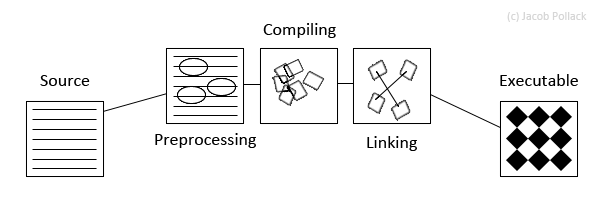
\includegraphics[scale=0.5]{terminator_figure.png}
\end{center}

\subsection{More Operators}

I know, I know. There are so many operators! Well blame CS 136 for introducing so many. The following operators are very important when it comes to memory.\\

We were introduced to a \emph{sizeof} operator that will determine the numbers of bytes to store a type. Keep in mind this operator is a compile-time operator and not a run-time operator. Example (for a 32-bit environment),\\

\lstset {
	language=c
}
\begin{lstlisting}
sizeof( int ) // => 4
\end{lstlisting}

We were also introduced to an address operator, \& that will return the address in hexadecimal of an identifier in memory. Note the single \& as oppose to the double \&\& to represent \textit{and}.\\

\lstset {
	language=c
}
\begin{lstlisting}
const int g = 9;

&g; // => address of g (&g).
\end{lstlisting}

\subsection{Hexadecimal, Decimal and Binary Notation}

In Computer Science we will often represent numbers in their hexadecimal, decimal and binary representations. It is important to understand what each form is and how to convert from one form to another. Let's begin with decimal.\\

Decimal notation is a way to represent a value in base 10. This notation should be very common to you as this is how we typically represent our values. We have 10 fingers and thus base 10 consists of the characters 0, 1, 2, 3, 4, 5, 6, 7, 8 and 9. With these 10 identifier (hence base 10) we are able to represent any value. For example,\\

$1204 = (1) \times (10^{3}) + (2) \times (10^{2}) + (0) \times (10^{1}) + (4) \times (10^{0})$\\

Hexadecimal notation is very common when referring to memory addresses in C. Nowadays your computer will likely have a 32-bit CPU or a 64-bit CPU. This is referring to the amount of memory addresses your computer can have. In a 32-bit environment we see that your computer can have $2^{32}$ memory addresses. Similarly in a 64-bit environment we see that your computer can have $2^{64}$ memory addresses. On the uBuntu VPS in CS 136 it uses a 32-bit environment and hence all mentions of data types will be with respect to a 32-bit environment. Now, back to hexadecimal. Hexadecimal is base 16 and consists of the characters 0, 1, 2, 3, 4, 5, 6, 7, 8, 9, A, B, C, D, E and F where A is 10, B is 11, C is 12, D is 13, E is 14 and F is 15 (base 10). Here is an example of the breakdown of a hexadecimal number,\\

0x00FFAE19 $= (15) \times (16^{5}) + (15) \times (16^{4}) + (10) \times (16^{3}) + (14) \times (16^{2}) + (1) \times (16^{1}) + (9) \times (16^{0})$\\

If you are a keen observer, you will notice that conversion between binary and hexadecimal is extremely easy since each hexadecimal character can be represented in 4 bits. Furthermore, two hexadecimal numbers can be represented in 8 bits. Example,\\

0xFF $= 11111111$ in binary.\\

This may not seem useful now, however it will become apparent once I start going over the review for how we store things in memory (it is probably the best chapter of this course).\\

Lastly, binary notation. It is extremely common when referring to the value that a memory address points to. An example of representing a value in binary is above (15 in hex is represented by 1111 binary).\\

Keep in mind that the following holds in C. Notice the use of 0x for hexadecimal.\\

\lstset {
	language=c
}
\begin{lstlisting}
int const a = 0xf;
int const b = 15;

( a == b ) // => true
\end{lstlisting}

\subsection{Memory}

Since a bit is such a small unit of measure. It became a standard that the smallest unit a Computer will use is a byte. Bits are still important, as every unit is measured in bits. However you will rarely (never in this course) need to access an individual bit. Here are some common units that we should be familiar with:

\begin{itemize}

\item Byte = 8 bits, $2^{8}$ possible values.
\item KiloByte = 1024 bytes.
\item MegaByte = 1024 kilobytes.
\item GigaByte = 1024 megabytes.
\item TeraByte = 1024 gigabytes.

\end{itemize}

In your computer you have something called \textbf{primary memory} (RAM) and \textbf{secondary memory} (hard drive, flash drives, etc.). Your primary memory is extremely fast in comparison to your secondary memory, however secondary memory is much cheaper to buy. I do not think we will be asked a question about this however we should know the difference.\\

Programs are launched into primary memory (random access memory) and disappear when the program is exited or when the computer shuts down. Secondary memory will remain persistent and hence often be used for storage.\\

I mentioned earlier the term \textbf{memory address}. A memory address is an identifier for one byte of memory. To access this byte you need to know its' address. Dave had an example in class where to call a friend, you need to know their phone number. You cannot call them without knowing their phone number, however when you have their phone number you can call them when ever you want. Memory is managed similarly with a few subtle differences. Memory addresses are typically represented in hexadecimal notation with the first byte as 0x00000000 and the last byte as 0xFFFFFFFF (on a 32-bit machine, remember all references are to a 32-bit machine) rather than decimal notation (like a phone number would be).\\

Now that we understand the bare bones of how memory works, let's recall how we declare a constant in C.\\

\lstset {
	language=c
}
\begin{lstlisting}
#include <stdio.h>

// Declaring a constant integer, a.
int const a = 9;

int main( void ) {
	printf( "The value of a is %d.\n", a ); // => 9
	printf( "The address in memory of a is 0x%08x.", &a ); // => 0x000002FF
	
	return 0;
}
\end{lstlisting}

Notice that the value of \emph{a} is 9, however the memory address of \emph{a} is 0x000002FF. This means that the bit representation of 9 is stored in memory addresses 0x000002FF, 0x00000300, 0x00000301 and 0x00000302. Recall an integer is 4 bytes and hence it will require 4 consecutive memory addresses. Those blocks of memory will look as follows.

\begin{center}
0x000002FF = [ 0 0 0 0 0 1 0 1 ]\\
0x00000300 = [ 0 0 0 0 0 0 0 0 ]\\
0x00000301 = [ 0 0 0 0 0 0 0 0 ]\\
0x00000302 = [ 0 0 0 0 0 0 0 0 ]\\
\end{center}

Note that this is using little-endianness. We do not need to know what this is however you should be aware that this is how it is stored in CS 136.

\subsection{The Sections of Memory}

This is one of the most important concepts to understand if you plan to design effective programs. The sections of memory. For the midterm we are responsible for knowing the following sections: \textbf{code}, \textbf{read-only}, \textbf{global data} and \textbf{stack}. The fifth section, \textbf{heap}, is not our responsibility and hence will not be referenced again.\\

\begin{center}
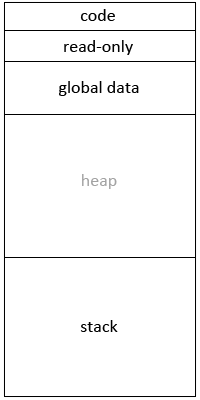
\includegraphics[scale=0.30]{memory_sections.png}
\end{center}

When your program is ran, the operating system will allocate x amount of bytes for your program. The smallest byte will be allocated to the code section and the largest byte will be allocated to the stack section. The code, read-only and global data sections grow from smaller addresses to bigger addresses and the stack grows from the biggest address to smaller addresses.\\

\lstset {
	language=c
}
\begin{lstlisting}
int const g = 10; // => the memory address of g could be 0x10.

int main( void  ) {
	int const a = 10; // => the memory address of a could be 0x200.
	int const b = 10; // => the memory address of b would be 0x196.
	int const c = 10; // => the memory address of c would be 0x192.
	
	return 0;
}
\end{lstlisting}

If you notice, these sections are constantly converging at each other. If the stack were to grow too big or the global data were to grow too big it would result in stack overflow. This is often occurs with infinite recursion or very deep recursion with poor overhead management.

\subsection{Overflow}

We got into a moderate amount of detail when it came to overflow. But you may ask yourself, what is overflow? Overflow is when the input value is greater than the maximum or minimum value determined by the amount of bytes allocated for a given type. To share an example, an integer is 4 bytes and hence has $2^{32}$ possible values. Since we want to represent negative numbers as well, an integer really only represents a number in the range of $2^{31}$ ... $2^{31} - 1$ (note the -1 to account for 0).\\

Now that we have determined the range that an integer can take on. What if we wanted to assign an integer to its' maximum value + 1? This would result in an overflow and the value would be some ambiguous number. Be careful when it comes to overflow! Choose the proper data types for the appropriate task or stress on the order of operations to minimize overflow. An example of overflow,\\

\lstset {
	language=c
}
\begin{lstlisting}
int const a = 1000000000; // => 1 billion, OK.
int const b = a * 3; // => 3 billion will overflow, PROBLEM.
\end{lstlisting}

\subsection{Characters in C}

You should be familiar with the \emph{char} data type. It is used to represent one byte. A character has $2^{8}$ possible values (-128 ... 127). In computers it is important to be able to communicate with another computer. There became a need to represent characters as numbers, hence the development of ASCII. It stands for American Standard Code for Information Interchange. Yes, I did just Wikipedia that however it may be important to know.\\

Each number from 0 ... 127 represents a character on the ASCII table. For example, 65 is the uppercase character A. Note, only characters 32 ... 126 (inclusive) are printable characters. Important to understand:

\begin{itemize}

\item Characters in ASCII are equivalent to numbers in C.
\item Characters are wrapped in single quotes, 'A' not double quotes "A" (invalid).

\end{itemize}

There is no difference between the following,\\

\lstset {
	language=c
}
\begin{lstlisting}
int const a = 65;
char const b = 'A';

( a == b ) // => true
\end{lstlisting}

An example of character arithmetic,\\

\lstset {
	language=c
}
\begin{lstlisting}
char to_lowercase( char const c ) {
	return ( ( ( c >= 'A' ) && ( c <= 'Z' ) ) ? c - 'A' + 'a' : c );
}
\end{lstlisting}

This example illustrates the power of treating characters as numbers to improve readability as well as some character arithmetic.

\subsection{Control Flow}

In C we have this fancy term called \textbf{control flow} which is used to model how a program is executed. When your program is ran, the program is given a specific \textbf{state} which includes the position at where the program currently is during its' execution. Operating systems invoke the \emph{main} function, it is the start of your program. There can only be \textbf{one} main function in your program! Moreover, the location is known as the \textbf{program counter} which stores the address of the machine code for the current instruction (it is in a yellow box in the notes).\\

Recall the control flow statement \emph{return}. This is used to \textbf{jump} back to where the function was called. It controls the flow of your program.

\subsection{The Call Stack}

In CS 136 we are expected to know what the \textbf{call stack} is. Suppose there is a function \textit{main} that calls a function \textit{f}, then that function calls a function \textit{g}. We say that \textit{f} is \textbf{pushed} onto the stack. Once it reaches a \textit{return} control flow statement, \textit{f} is \textbf{popped} from the stack. This history is known as the call stack.\\

A \textbf{stack frame} consists of the arguments passed to the function, local variables/constants and the return address for the function. When a global constant is declared it is put into the read-only section of memory. Local constants are put into the stack section of memory. When the stack is popped, the local constants disappear however the global constants remain persistent throughout the execution of the program. As of right now, all arguments are copies of their value in memory -- important to be aware of this.\\

Here is a sample set of functions,\\

\lstset {
	language=c
}
\begin{lstlisting}
int g( int const x ) {
	return x + 3;
}

int f( int const x ) {
	int const a = ( x * 2 ) + g( x );
}

int main( void  ) {
	const int result = f( 5 );
	
	// ...
	
	return 0;
}
\end{lstlisting}

The call stack would look as follows before a stack frame is popped,\\

\lstset {
	language=c
}
\begin{lstlisting}
/**
 * ====================
 * g:
 * 	x: 5
 * 	return addr: f:6
 * ====================
 * f:
 * 	x: 5
 * 	a: ?
 * 	return addr: main:10
 * ====================
 * main:
 * 	result: ?
 * 	return addr: OS
 * ====================
 */
\end{lstlisting}

The call stack is stored in the stack section of our memory model. This is important! If you recall what I stated earlier about stack overflow and how it occurs. You should now see why. Here is an overview of all of the memory sections we are responsible for,\\

\lstset {
	language=c
}
\begin{lstlisting}
int const g = 9; // => &g is global data.

int main( void ) { // => &main is code.
	int const s = 9; // => &s is stack.
	
	return 0;
}
\end{lstlisting}

\subsection{Pointers}

Pointers are a very powerful tool in a C programmers belt. This is arguably one of the toughest concepts to grasp however it is definitely one of the most rewarding. I will spend some time reviewing what pointers are and illustrating some examples. In my opinion, it is essential for you to understand what pointers are and how to use them. I am nearly certain there will be questions on the midterm and final involving pointers.\\

We have taken a look at the address of operator (\&) which will give us the memory address of an identifier. But how do we point to a specific memory address? Well, we use pointers! Declaring a pointer allows us to access specific memory addresses which can be extremely useful and extremely dangerous.\\

\lstset {
	language=c
}
\begin{lstlisting}
// Declaration of a constant integer, i.
int const i = 9;

// Declaration of a pointer to a constant integer, pi.
int const *pi = &i;
\end{lstlisting}

Observe the declaration of the pointer. We use the * operator to mean "points to". You would read the declaration as, "\textit{pi} is a pointer to a constant integer \textit{i}.". Yes, * is also the multiplication operator however in C it has multiple uses. Note, the value of the pointer is a hexadecimal address.\\

\begin{center}
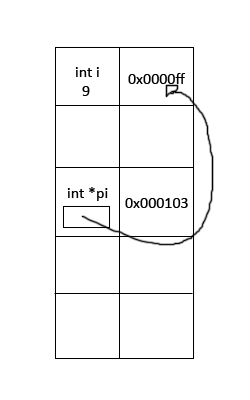
\includegraphics[scale=0.35]{pointer_example.png}
\end{center}

Seeing as the value of a pointer is a hexadecimal address, can you guess what the size of a pointer is? No matter what data type, a pointer will always have a size of 4 bytes. This is important as we will take advantage of this fact to reduce stack overhead.\\

To get the value of which \textit{pi} points to we need to use a special operator called the \textbf{indirection operator} (*), or more commonly known as \textbf{derefencing} \textit{pi}. I know this is confusing but bare with me! The star (*) is used to multiply, point and dereference.\\

\lstset {
	language=c
}
\begin{lstlisting}
int main( void ) {
	// Declaration of a constant integer, i.
	int const i = 9;

	// Declaration of a pointer to a constant integer, pi.
	int const *pi = &i;

	printf( "i = %d\n", i ); // => 9
	printf( "i = 0x%08x\n", &i ); // => 0x00000103
	printf( "*pi = %d\n", *pi ); // => 9
	printf( "pi = 0x%08x\n", pi ); // => 0x00000103
	printf( "&pi = 0x%08x", &pi ); // => 0x000000FF
	
	return 0;
}
\end{lstlisting}

Note that the following is a complicated but completely valid expression in C where x is a pointer to some integer,\\

\lstset {
	language=c
}
\begin{lstlisting}
*x * *x
\end{lstlisting}

What this example is saying is that, dereference x and square it. This can get even more complicated as we are able to declare pointers to pointers.\\

\lstset {
	language=c
}
\begin{lstlisting}
int main( void ) {
	// Declaration of a constant integer, i.
	int const i = 9;

	// Declaration of a pointer to a constant integer, pi.
	int const *pi = &i;
	
	// Declaration of a pointer to a pointer to a constant integer, ppi.
	int const **ppi = &pi;

	printf( "i = %d\n", i ); // => 9
	printf( "&i = 0x%08x\n", &i ); // => 0x00000107
	printf( "*pi = %d\n", *pi ); // => 9
	printf( "pi = 0x%08x\n", pi ); // => 0x00000107
	printf( "&pi = 0x%08x", &pi ); // => 0x00000103
	printf( "*ppi = 0x%08x\n", *ppi ); // => 0x00000107
	printf( "**ppi = %d\n", **ppi ); // => 9
	printf( "ppi = 0x%08x\n", ppi ); // => 0x00000103
	printf( "&ppi = 0x%08x", &ppi ); // => 0x000000ff
	
	return 0;
}
\end{lstlisting}

You should also be aware that we can have pointers as parameters.\\

\lstset {
	language=c
}
\begin{lstlisting}
int some_func( int const *pi, int const **ppi ) {
	// ...
}
\end{lstlisting}

Keep in mind that to pass a pointer as an argument you must pass the address of the identifier using the address operator (\&).\\

There are two special types of pointers. There is a \textit{null} pointer and a \textit{void} pointer. If a pointer points to \textit{null} then it is considered as invalid or that it points to nothing. It is required that we check for \textit{null} pointers in our pre condition of any given function that is passed a pointer as an argument. On the other hand, if a pointer is a \textit{void} pointer (\textit{void *}) then it can accept a memory address where the data type is unknown. You cannot dereference a \textit{void} pointer however you are able to modify the memory it points to which will become useful later.\\

We were introduced to function pointers which are actually very useful. Function pointers are pointers that point to functions. This gives us the ability to pass functions as arguments to other functions. Consider the following.\\

\lstset {
	language=c
}
\begin{lstlisting}
int sub1( int i ) {
	return ( i - 1 );
}

int main( void ) {
	int ( *sub1_alias )( int ) = sub1;
	
	int const five = sub1( six );
	int const four = sub1_alias( five );
	
	return 0;
}
\end{lstlisting}

Note there is no address of operator when pointer to a function.\\

Another very useful cool thing with pointers is they can be used to reduce stack overhead. This becomes very apparent when passing structures as arguments. If you call, arguments are copied to the stack frame. If you have a very large structure it will copy it every time you call the function. If you are using recursion, this will create a lot of stack overhead. To avoid this, we pass pointers to structures. First, consider the following.\\

\lstset {
	language=c
}
\begin{lstlisting}
struct struct_1 {
	int x;
	char y;
	char z;
};

struct struct_2 {
	char y;
	int x;
	char z;
};

printf( "The size of struct_1 is: %d\n", sizeof( struct_1 ) ); // => 8
printf( "The size of struct_2 is: %d\n", sizeof( struct_2 ) ); // => 12
\end{lstlisting}

This is called structure padding. The processor deals with data types in multiples of 4 bytes. This is to improve efficiency. The bytes not used by the structure will be filled with empty bytes. To pass structures as arguments we do the following.\\

\lstset {
	language=c
}
\begin{lstlisting}
struct posn {
	int x;
	int y;
};

int some_func( struct posn *p ) {
	return ( *p ).x + ( *p ).y;
}

// ... or alternatively using the right arrow selection operation.

int some_func( struct posn *p ) {
	return p->x + p->y;
}
\end{lstlisting}

\newpage
\section{Imperative C: Module 05}

Once module 05 was released there was the "Computer Science equivalent" of a standing ovation in Dave's class. If you recall from the beginning of module 01 I mentioned that we will be revisiting the imperative paradigm soon. Well, this is that moment in time.\\

Using an \textbf{imperative paradigm} is the process of using control flow to manipulate state, using a series of statement to describe how to achieve an outcome\footnote{There is a fantastic example that Dave illustrates using Kraft Dinner. I hope all of you are lucky enough to get a chance to see his example!}.

\subsection{Imperative Paradigm in Racket}

There are three fancy functions that we are introduced to in Racket that allow us to use control flow to manipulate state. These functions are \emph{begin}, \emph{printf} and \emph{set!}. See their respective documentation for further information on those individual functions. Here is an example using all three in a favorite color module.\\

\lstset {
	language=Lisp
}
\begin{lstlisting}
#lang racket ; favorite-color.rkt

(define favorite-color 'blue)

(define (guess-color color)
	(cond
		[(symbol=? color favorite-color) (begin (printf "You guessed correctly!")
		                                        (set! favorite-color 'green)
		                                        #t)]
		[else (printf "You guessed incorrectly.") #f]))
\end{lstlisting}

Note the use of the \textbf{implicit \emph{begin}} in the else block. \emph{Begin} is similar to \emph{local} in the aspect that they can both be implicitly written in Racket.\\

Observe that \emph{printf} is outputting to the console and producing \emph{void}. We say that \emph{printf} has a \textbf{side effect}, it being that \emph{printf} is outputting to the console. It is extremely important to document side effects in the design recipe. Keep in mind side effects are only in an imperative paradigm - you cannot have a side effect in a functional paradigm.\\

Note, there can exist functions that only have side effects! These functions are declared with \emph{void}. Example,\\

\lstset {
	language=c
}
\begin{lstlisting}
void hello_world( void ) {
	printf( "Hello world!\n" );
	
	return; // Optional in VOID functions.
}
\end{lstlisting}

Here is an example of the documentation for a function that will square a number, x and output to the console "You squared me!":\\

\lstset {
	language=Lisp
}
\begin{lstlisting}
; square_x: Int -> Int
;	Purpose: Consumes an integer, x and produces the value of
;            x squared.
; PRE: true
; POST: - produces an integer >= 0,
;       - Side Effect: outputs "You squared me!".
(define (square_x x)
	(printf "You squared me!")
	(* x x))
\end{lstlisting}

\subsection{Imperative Paradigm in C}

Similar to Racket, you can program imperatively in C. Note there is a key difference between \emph{printf} in Racket and in C. In Racket it produces \emph{void} however in C it returns the number of characters outputted to the console. The return type of \emph{printf} in C is \emph{int}.\\

In C we have curly braces (\{ \}). These braces are also known as a compound statement, or more commonly, a C block. A C block behaves similarly to \emph{begin} in Racket with one key difference. In Racket it will evaluate every statement within the compound statement, however in C it requires a control flow statement to tell the block to stop evaluating. This control flow statement is called \emph{return} (which you should be familiar with).

\subsection{Control Flow Statements}

In an imperative paradigm we are introduced to a few new control flow statements. Those statements being: \emph{if}, \emph{for}, \emph{while}, \emph{switch}, \emph{continue} and \emph{break}. We are responsible for knowing the behavior of each of these control flow statements with the exception of \emph{switch}.\\

The \emph{if} statements is setup as follows.\\

\lstset {
	language=c
}
\begin{lstlisting}
if (exp) {
	// ... true.
} else if (exp) {
	// ... true.
} else {
	// ... false.
}

// ... or alternatively

if (exp)
	// true.
else
	// false.
\end{lstlisting}

I am showing the second method of setting up an \emph{if} statement however it is extremely bad practice and should be avoided at all costs! Consider the following.\\

\lstset {
	language=c
}
\begin{lstlisting}
if (exp)
	// ... true.
	if (exp)
		// ... true.
else
	// ... false.
\end{lstlisting}

But is the \emph{else} applied to the first or the second if statement? In general and with respect to CS 136 - we should avoid this. Keep in mind you can have a long chain of \textit{if}/\textit{else if}/\textit{else} statements. Here is yet another example of a function \emph{sum} that will produce the sum of 0 ... n.\\

\lstset {
	language=c
}
\begin{lstlisting}
int sum( int n ) {
	if ( 0 == n ) {
		return n;
	} else {
		return n + sum( n - 1 );
	}
}

// ... or alternatively

int sum( int n ) {
	if ( 0 == n ) {
		return n;
	}
	
	return n + sum( n - 1 );
}
\end{lstlisting}

Note that you can have multiple control flow statements. These are used to "control the flow" of your function. There is an extremely common error this semester on Piazza. This error is "reached end of non-void function". This error is caused because you are not including the proper control flow statements. Consider the following.\\

\lstset {
	language=c
}
\begin{lstlisting}
int do_something( int n ) { // BAD BAD BAD!!!
	if ( 0 <= n ) {
		return n;
	}
	
	// ... some more code, but oops - no return?!
}

int do_something( int n ) { // OK!
	if ( 0 <= n ) {
		return n;
	}
	
	return n * -1;
}
\end{lstlisting}

What would happen if we called the function \emph{do\_something} and passed it -1? The function would spit out the error "reached end of non-void function". To avoid this, make the appropriate corrections.\\

\subsection{Mutation}

So far all we have been able to use is constants. Recall, constants are immutable, meaning once they are declared they can never be changed throughout the execution of the program. We are finally, emphasis on finally, introduced to variables. Unlike constants, once a variable is \textbf{initialized} to a value it can be re-assigned (overwritten in memory) to a new value. Let's consider the following.\\

\lstset {
	language=c
}
\begin{lstlisting}
int a = 9; // Note the absence of 'const'.

printf( "a = %d\n", a ); // => 9

a = 8; // Mutating a.

printf( "a = %d\n", a); // => 8
\end{lstlisting}

Remark that we can mutate a as many times as we want throughout our program.

\subsection{Assignment Operator}

In C the \textbf{assignment operator =} (not ==, the equivalent operator) is used to assign a value to an identifier. If you are a Math student you will likely find the following confusing (however if you are reviewing for the midterm I really hope you do not!).\\

\lstset {
	language=c
}
\begin{lstlisting}
x = y;

y = x;
\end{lstlisting}

The first line is assignment the value of y to x. The third line is assignment the value of x to y. Note these are not equivalent operations! In variable declarations we say that the variable \emph{var} is \textbf{initialized} to a value.\\

The assignment operator performs two actions. In the example above (line 1), x is being assigned to y. After it overwrites x in memory, it will return the value of y. Here is an example of very confusing code.\\

\lstset {
	language=c
}
\begin{lstlisting}
int x = 10;
int y = 11;

printf( "%d\n", ( x = ( y + 1 ) ) ); // => Outputs 22.
\end{lstlisting}

\textbf{Remark} that the assignment operator is performing a side effect! It is overwriting a value in memory with a new value. These mutations should be documented appropriately.

\subsection{Static Storage}

Right now you should be aware that \emph{static} gives global constants/variables modular scope. But what happens if we declare a \emph{static} local variable? Static storage stores local variables in the global data section of memory while keeping its scope local to the function that the static local variable was declared in. This may be confusing, however take a look at the following example.\\

\lstset {
	language=c
}
\begin{lstlisting}
int func( void ) {
	static int total_func_called = 0;
	
	total_func_called = total_func_called + 1;
	
	return total_func_called;
}

func(); // => 1
func(); // => 2
func(); // => 3
func(); // => 4
\end{lstlisting}

This function will \emph{return} the amount of times the function has been called. Static storage is very useful as you have probably noticed on assignment five.

\subsection{Uninitialized Data}

In C you are able to declare variables without an initial value. This is called an uninitialized variable and looks as follows.\\

\lstset {
	language=c
}
\begin{lstlisting}
int i;
\end{lstlisting}

Uninitialized variables are considered bad practice. However, if you insist on doing it then there are some rules. If you declare a global variable then it will be automatically initialized to 0 (if no value is specified), however if you declare a variable on the stack it will be initialized to some garbage value (some arbitrary value from a previous stack frame). You must \textbf{always} initialize variables on the stack.

\subsection{Assignment Shortcuts}

Ha! I bet this section caught someones eye. As programmers we are extremely lazy. Conveniently, C provides us with ways to assign values to variables. You should know how to use the following however I am listing them here just to recap!\\

\lstset {
	language=c
}
\begin{lstlisting}
int x = 10;
int y = 11;

x = x + 1;
y = y + 1;

// ... is equivalent to.

x += 1;
y += 1;

// ... is equivalent to.

x++; // returns the value of x then increments x by 1.
y++; // returns the value of y then increments y by 1.

// ... or.

++x; // increments the value of x by 1 then returns the value of x.
++y; // increments the value of y by 1 then returns the value of y.
\end{lstlisting}

The thing to notice here is the prefix and suffix notation for the ++. This is an operator that will increment the existing value in memory by 1.

\subsection{Examples of Mutation}

Now that we have learned what imperative programming is, it is time to show you some classic examples of imperative programming. Consider the following function that will swap two values.\\

\lstset {
	language=c
}
\begin{lstlisting}
void swap( int * const x, int * const y ) {
	int const temp = *x;
	
	*x = *y;
	*y = temp;
}
\end{lstlisting}

Note the use of pointers and a temporary constant \emph{temp}. Without pointers the swapped values would disappear once the stack frame is popped from the call stack. Let's take a look at another example using structures.

\lstset {
	language=c
}
\begin{lstlisting}
void reflect( struct posn * const p ) {
	int const temp = p->x;
	
	p->x = p->y;
	p->y = temp;
}
\end{lstlisting}

This function reflects a point in the line $y = x$.\\

If you noticed in the previous two examples I am using the keyword \emph{const} in a weird place. Here is how it would be read in example 2, "p is a constant pointer pointing to a struct posn". Here are all the possible combinations (important):\\

\lstset {
	language=c
}
\begin{lstlisting}
int *p; // P is a pointer to an integer.

int const *p; // P is a pointer to a constant integer.

int * const p; // P is a constant pointer to an integer.

int const * const p; // P is a constant pointer to a constant integer.
\end{lstlisting}

The only difference between a constant pointer and a pointer is the value that \emph{p} points to cannot change. This is exactly what you would expect \emph{const} to do.

\subsection{Looping: Iteration}

Iteration is the imperative way of doing recursion. There are cases where recursion may seem more "logical" to look at, however iteration is the way CS 136 wants us doing things nowadays. Consider the following introductions of the \emph{while} loop, \emph{do-while} loop and the \emph{for} loop.\\

\lstset {
	language=c
}
\begin{lstlisting}
do {
	// ... some code to be executed indefinitely once.
} while ( exp );

while ( exp ) {
	// ... do something involving the expression.
}

for ( declaration; expression; mutation on the declaration ) {
	// ... do something.
}
\end{lstlisting}

These two control flow statements will iterate until the expression is false. Note, you can nest loops. Consider the following function that will output a chess board of size n in ASCII.\\

\lstset {
	language=c
}
\begin{lstlisting}
void make_chessboard( int const n ) {
	for ( int r = 0; r < n; r++ ) {
		for ( int c = 0; c < n;  c++ ) {
			const int is_black = ( ( ( c - r ) % 2 ) == 0 );
			
			if ( is_black ) {
				printf( "**" );
			} else {
				printf( "  " );
			}
		}
		
		printf( "\n" );
	}
}
\end{lstlisting}

\newpage
\section{Praise}

I tried to keep this section a secret. However, if you have made it this far in my review notes then you are awesome! I wish you best of luck on your midterm. If you have any feedback please do not hesitate to contact me.\\

Live long and prosper *separates fingers*!

\newpage
\section{Exercises}

These exercises are based on material that I feel we as a class struggled with. The professors conveniently posted the assignment averages and question averages of all the students. I picked concepts with the lowest average to create exercises for. \textbf{These exercises should not replace incomplete assignment questions - do those first}. Have fun completing these!\\

There are no test cases or solutions to any of these problems - it is your job to come up with your own test cases. If you need help with any of these questions refer to course material (or Piazza?).

\subsection{In Racket}

The following exercises are to be completed in Racket. Pay close attention to the restrictions on the questions!

\subsubsection{Structures}

\textbf{1.} Write a function \emph{reshuffle\_bst} that consumes a valid BST. This function should find the smallest node and make it the root node. It should handle all appropriate shuffling to keep the BST ordered. It will produce the new, shuffled BST. Keep in mind a BST is defined as follows. \textbf{You must implement this using recursion}.\\

\lstset {
	language=Lisp
}
\begin{lstlisting}
(struct bst-node (key val left right) #:transparent)
\end{lstlisting}

\noindent
\textbf{2.} Write a function \emph{bst-height} that will consume a valid BST and produce the height of the BST. You may assume an empty BST has a height of 0.\\

\noindent
\textbf{3.} Write a function \emph{bst-full} that will consume a valid BST and produce \#t if the BST is full, meaning every node in the tree has two children that are either both non-empty or both empty, otherwise \#f.\\

\noindent
\textbf{4.} Write a function \emph{posn-equal?} that will consume two valid \emph{posn}s and produce \#t if they are they same points on the euclidean plane, otherwise \#f.\\

\subsubsection{Lists}

\textbf{1.} Write a function \emph{convert-to-assoc-lst} that will consume a non-empty list. It will produce an associative list starting from index 0 treating every element of the consumed list as a value. \textbf{You cannot use recursion}. Example:\\

\lstset {
	language=Lisp
}
\begin{lstlisting}
(equal? (convert-to-assoc-lst (list 1 2)) '((0 1) (1 2))) ; => #t
\end{lstlisting}

\noindent
\textbf{2.} Write a function \emph{to-base-x} that will consume two integers, n and b where n is a number and b is a base. It will produce all the digits in proper order of n converted to base b. Example:\\

\lstset {
	language=Lisp
}
\begin{lstlisting}
(equal? (to-base-x 9 2) '(1 0 1)) ; => #t
\end{lstlisting}

\noindent
\textbf{3.} Write a function that consumes a non-empty list and produces the same list reversed. \textbf{You cannot use abstract list functions, you must use recursion}.

\subsubsection{Other}

\textbf{1.} For this question you are expected to use mutation (\emph{set!}). You will have a lot of freedom on the implementation for this question so be creative. First, write a function \emph{give-backpack} that consumes nothing. It has a side effect that if you do not already have a backpack it will create one for you and output "Congratulations, a free backpack!", otherwise it will output to the console "You fool, you cannot wear two backpacks!" and remove your current backpack.\\

The second function you need to make is called \emph{give-me-something}. It consumes nothing and produces nothing. If you have a backpack, it will add a random object to your backpack (a number) and output what it added followed by a new line, otherwise it will output "You do not have a backpack!".\\

The contracts are as follows.\\

\lstset {
	language=Lisp
}
\begin{lstlisting}
; give-backpack: Void -> Void

; give-me-something: Void -> Void
\end{lstlisting}

\subsection{In C}

The following exercises are to be completed in C (C99). Pay close attention to the restrictions on the questions!

\subsubsection{Structures}

\textbf{1.} Write the declaration for a function \emph{minimal\_posn\_overhead}. It is passed one argument, a struct \emph{posn}. Write it in such a way that stack overhead is reduced as much as possible.\\

\noindent
\textbf{2.} Write a function \emph{is\_posn\_equal} that is passed two arguments that are \emph{struct posn}s. This function will return true if they are the same point on the euclidean plane, otherwise false.\\

\noindent
\textbf{3.} Write a function \emph{is\_orthogonal\_set} that is passed two arguments. The first and second arguments are both \emph{struct Vectors}. It will return true if both vectors form an orthogonal set in $R^{2}$, otherwise false. Where a \emph{struct Vector} is defined as.\\

\lstset {
	language=Lisp
}
\begin{lstlisting}
struct Vector {
	int x;
	int y;
};
\end{lstlisting}

\noindent
\textbf{4.} Write a function \emph{key\_exists} that is passed two arguments, an integer, \textit{i} and a valid BST, \textit{abst}. This function will return true if the key exists, otherwise false. Keep in mind that an empty bst points to NULL and the BST structure is defined as follows. \textbf{You must implement this using recursion}.\\

\lstset {
	language=c
}
\begin{lstlisting}
struct bst_node {
	int key;
	int val;
	struct bst *left;
	struct bst *right;
};
\end{lstlisting}

The declaration of the function is as follows.\\

\lstset {
	language=c
}
\begin{lstlisting}
bool key_exists( int const i, struct bst * const pbst );
\end{lstlisting}

\subsubsection{Loops}

\textbf{1.} Write a function \emph{make\_chessboard} that is passed two arguments, x1 and x2 where x1 and x2 are both integers. It has a side effect that will output a chessboard of size x1 by x2 (width by length). Black squares are "**" and white squares are "  " (note the double space). It will return void. \textbf{You must implement this using loops}.

\subsubsection{Memory Model}

\textbf{1.} Figure out where each constant, variable and function declaration is stored in memory. For every constant and variable declared locally to main, determine there exact hexadecimal memory address assuming the address of s1 = 0x300.\\

\lstset {
	language=c
}
\begin{lstlisting}
int const g1 = 9;
int g2 = 1337;
static g3 = 7331;

int main( void ) {
	int const s1 = 100;
	
	int *ps = &s1;
	
	char c1 = 'J';
	char c2 = 'P';
	
	char *pc = &c1;
	
	return 0;
}
\end{lstlisting}

\noindent
\textbf{2.} Draw the memory block (assuming little-endianness) of the following 32-bit integer declaration. Hint, be careful this is a signed integer!\\

\lstset {
	language=c
}
\begin{lstlisting}
int const g = -255;
\end{lstlisting}

\subsubsection{Pointers}

\textbf{1.} Write a function \emph{max\_val} that is passed three arguments. The first two arguments are integers i, n and the third argument is a function, f. Max val will return max(f(i), f(n)).\\

\noindent
\textbf{2.} Write functions \emph{pinc}, \emph{pdec} and \emph{sinc}, \emph{sdec} that will perform the exact same as ++var, --var and var++, var--. Hint, use pointers.

\subsubsection{Bitwise}

\textbf{1.} Write a function \emph{flip\_bits} that is passed one argument. This argument is a character that must be $>= 0$. This function will flip all 8 bits in the character and return an integer with the new binary representation of the character. \textbf{You cannot use the built in C function XOR, you must use iteration and other bitwise operators (bit shifters, \& and $|$ are permitted)}. Hint, your mask \emph{could} be 0x80.\\

\lstset {
	language=c
}
\begin{lstlisting}
assert( flip_bits( 9 ) == 11110110 ); // Note 9 is 1001 in binary.
\end{lstlisting}

\subsubsection{Errors}

\textbf{1.} What does "reached end of non-void function" mean?\\

\noindent
\textbf{2.} What does "bus error" mean?\\

\noindent
\textbf{3.} Consider the following function. Why is the following solution wrong?\\

\lstset {
	language=c
}
\begin{lstlisting}
/**
 * sum( n ): Consumes one argument, n and returns the sum
 *           from 0 ... n.
 * PRE: n >= 0
 * POST: returns an integer >= 0
 */
int sum( int n ) {
	return ( ( 0 == n ) ? n : sum( n - 1 ) );
}
\end{lstlisting}

\noindent
\textbf{4.} Consider the following function. Identify why the solution did not receive full marks?\\

\lstset {
	language=c
}
\begin{lstlisting}
#include <stdio.h>

/**
 * sum( void ): Consumes no arguments. Returns the amount of times
 *              this function has been called.
 * PRE: true
 * POST: - returns an integer >= 0
 */
int func_counter( void ) {
	static int counter = 0;
	
	counter += 1;	
	
	printf( "This function has been called %d times.\n", counter );
	
	return counter;
}
\end{lstlisting}

\noindent
\textbf{4.} Consider the following function. Identify the error.\\

\lstset {
	language=c
}
\begin{lstlisting}
#include <stdio.h>

/**
 * sum( n ): Consumes one argument, n and returns the sum
 *           from 0 ... n.
 * PRE: n >= 0
 * POST: returns an integer >= 0
 */
int sum( int n ) {
	return ( is_zero( n ) ? n : ( n + sum( n - 1 ) ) );
}

static int is_zero( int n ) {
	return ( 0 == n );
}
\end{lstlisting}

\noindent
\textbf{5.} Consider the following function. Identify the error.\\

\lstset {
	language=c
}
\begin{lstlisting}
#include <stdio.h>

int main( void ) {
	int i = 9;
	int k = 10;
	int * const p = &i;
	
	printf( "i = %d\n", *p );
	
	pi = &j;
	
	printf( "j = %d\n", *p );
	
	return 0;
}
\end{lstlisting}

\subsubsection{Word Problems}

\textbf{1.} What is the difference between a function declaration and a definition?

~\\
\noindent
\textbf{2.} What is static storage?\\

\noindent
\textbf{3.} What is the difference between the read-only and global data section of memory?\\

\noindent
\textbf{4.} What is the difference between a standard library and a library you create?\\

\noindent
\textbf{5.} Convert 0xff from hexadecimal to base 2 (binary) and base 10 (decimal). What observations can you make of the binary representation.

~\\
\noindent
\textbf{6.} What is the size of a memory address on a 32-bit machine? How about a 64-bit machine? If I were to declare an integer on a 16-bit machine, what would its size be?\\

\noindent
\textbf{7.} Why is C++ a pun?\\

\noindent
\textbf{8.} List four of the five sections of memory.\\

\noindent
\textbf{9.} Explain in detail the steps that occur behind the scenes when you hit "Run" in gedit using RunC.\\

\noindent
\textbf{10.} What happens if I do not initialize a variable on the stack?\\

\end{document}
